\documentclass[oneside,openany,headings=optiontotoc,11pt,numbers=noenddot]{scrreprt}

\usepackage[a4paper]{geometry}
\usepackage[utf8]{inputenc}
\usepackage[T1]{fontenc}
\usepackage{lmodern}
\usepackage[ngerman]{babel}
\usepackage{ngerman}

\usepackage[onehalfspacing]{setspace}

\usepackage{fancyhdr}
\usepackage{fancybox}

\usepackage{rotating}
\usepackage{varwidth}

%Struktogramme
\usepackage[german,curves]{struktex}

\usepackage{pdflscape}
\usepackage{changepage}
\usepackage{graphicx}
\usepackage[bottom]{footmisc}
\usepackage{transparent}
\usepackage{graphbox}
\graphicspath{
	{Pics/PDFs/}
	{Pics/JPGs/}
	{Pics/PNGs/}
}
\usepackage{caption}
\usepackage{wrapfig}
\usepackage{marginnote}
\usepackage{tabularx}
\usepackage{dashrule}
\usepackage{soulutf8}
\usepackage{hhline}
%arydshln suppresses vertical lines in table
%\usepackage{arydshln}
\usepackage{multirow}
\usepackage{enumerate}
\usepackage[hidelinks]{hyperref}
\usepackage{listings}

\usepackage[table]{xcolor}
\usepackage{array}
\usepackage{enumitem,amssymb,amsmath}
\usepackage{interval}
\usepackage{cancel}
\usepackage{stmaryrd}
\usepackage{wasysym}
\usepackage{polynom}
\usepackage{diagbox}
\usepackage{dashrule}
\usepackage{framed}
\usepackage{mdframed}
\usepackage{karnaugh-map}
\usepackage{pdfpages}

\usepackage{blindtext}

\usepackage{eso-pic}

\usepackage{amssymb}
\usepackage{eurosym}

\usepackage[pages=some]{background}
\pagestyle{headings}
\renewcommand{\headrulewidth}{0.2pt}
\renewcommand{\footrulewidth}{0.2pt}
\newcommand*{\underdownarrow}[2]{\ensuremath{\underset{\overset{\Big\downarrow}{#2}}{#1}}}
\setlength{\fboxsep}{5pt}
\newcommand{\explainBelow}[3]{\underbrace{#1}_{\parbox{\widthof{#3}}{\footnotesize\raggedright #2}}}
\newcommand{\explainAbove}[3]{\overbrace{#1}^{\parbox{\widthof{#3}}{\footnotesize\raggedright #2}}}
\newcommand\footnoteref[1]{\protected@xdef\@thefnmark{\ref{#1}}\@footnotemark}


% Codestyle defined
\definecolor{codegreen}{rgb}{0,0.6,0}
\definecolor{codegray}{rgb}{0.5,0.5,0.5}
\definecolor{codepurple}{rgb}{0.58,0,0.82}
\definecolor{backcolour}{rgb}{0.95,0.95,0.92}
\definecolor{deepgreen}{rgb}{0,0.5,0}
\definecolor{darkblue}{rgb}{0,0,0.65}
\definecolor{mauve}{rgb}{0.40, 0.19,0.28}
\colorlet{exceptioncolour}{yellow!50!red}
\colorlet{commandcolour}{blue!60!black}
\colorlet{numpycolour}{blue!60!green}
\colorlet{specmethodcolour}{violet}

%Neue Spaltendefinition
\newcolumntype{L}[1]{>{\raggedright\let\newline\\\arraybackslash\hspace{0pt}}m{#1}}
\newcolumntype{M}{>{\centering\arraybackslash}X}
\newcommand{\cmnt}[1]{\ignorespaces}
%Textausrichtung ändern
\newcommand\tabrotate[1]{\rotatebox{90}{\raggedright#1\hspace{\tabcolsep}}}

%Intervall-Konfig
\intervalconfig {
	soft open fences
}

%Bash
\lstdefinestyle{BashInputStyle}{
	language=bash,
	basicstyle=\small\sffamily,
	backgroundcolor=\color{backcolour},
	columns=fullflexible,
	backgroundcolor=\color{backcolour},
	breaklines=true,
}
%Java
\lstdefinestyle{JavaInputStyle}{
	language=Java,
	backgroundcolor=\color{backcolour},
	aboveskip=1mm,
	belowskip=1mm,
	showstringspaces=false,
	columns=flexible,
	basicstyle={\footnotesize\ttfamily},
	numberstyle={\tiny},
	numbers=none,
	keywordstyle=\color{purple},,
	commentstyle=\color{deepgreen},
	stringstyle=\color{blue},
	emph={out},
	emphstyle=\color{darkblue},
	emph={[2]rand},
	emphstyle=[2]\color{specmethodcolour},
	breaklines=true,
	breakatwhitespace=true,
	tabsize=2,
}
%Python
\lstdefinestyle{PythonInputStyle}{
	language=Python,
	alsoletter={1234567890},
	aboveskip=1ex,
	basicstyle=\footnotesize,
	breaklines=true,
	breakatwhitespace= true,
	backgroundcolor=\color{backcolour},
	commentstyle=\color{red},
	otherkeywords={\ , \}, \{, \&,\|},
	emph={and,break,class,continue,def,yield,del,elif,else,%
		except,exec,finally,for,from,global,if,import,in,%
		lambda,not,or,pass,print,raise,return,try,while,assert},
	emphstyle=\color{exceptioncolour},
	emph={[2]True,False,None,min},
	emphstyle=[2]\color{specmethodcolour},
	emph={[3]object,type,isinstance,copy,deepcopy,zip,enumerate,reversed,list,len,dict,tuple,xrange,append,execfile,real,imag,reduce,str,repr},
	emphstyle=[3]\color{commandcolour},
	emph={[4]ode, fsolve, sqrt, exp, sin, cos, arccos, pi,  array, norm, solve, dot, arange, , isscalar, max, sum, flatten, shape, reshape, find, any, all, abs, plot, linspace, legend, quad, polyval,polyfit, hstack, concatenate,vstack,column_stack,empty,zeros,ones,rand,vander,grid,pcolor,eig,eigs,eigvals,svd,qr,tan,det,logspace,roll,mean,cumsum,cumprod,diff,vectorize,lstsq,cla,eye,xlabel,ylabel,squeeze},
	emphstyle=[4]\color{numpycolour},
	emph={[5]__init__,__add__,__mul__,__div__,__sub__,__call__,__getitem__,__setitem__,__eq__,__ne__,__nonzero__,__rmul__,__radd__,__repr__,__str__,__get__,__truediv__,__pow__,__name__,__future__,__all__},
	emphstyle=[5]\color{specmethodcolour},
	emph={[6]assert,range,yield},
	emphstyle=[6]\color{specmethodcolour}\bfseries,
	emph={[7]Exception,NameError,IndexError,SyntaxError,TypeError,ValueError,OverflowError,ZeroDivisionError,KeyboardInterrupt},
	emphstyle=[7]\color{specmethodcolour}\bfseries,
	emph={[8]taster,send,sendMail,capture,check,noMsg,go,move,switch,humTem,ventilate,buzz},
	emphstyle=[8]\color{blue},
	keywordstyle=\color{blue}\bfseries,
	rulecolor=\color{black!40},
	showstringspaces=false,
	stringstyle=\color{deepgreen}
}

\lstset{literate=%
	{Ö}{{\"O}}1
	{Ä}{{\"A}}1
	{Ü}{{\"U}}1
	{ß}{{\ss}}1
	{ü}{{\"u}}1
	{ä}{{\"a}}1
	{ö}{{\"o}}1
}

% Neue Klassenarbeits-Umgebung
\newenvironment{worksheet}[3]
% Begin-Bereich
{
	\newpage
	\sffamily
	\setcounter{page}{1}
	\ClearShipoutPicture
	\AddToShipoutPicture{
		\put(55,761){{
				\mbox{\parbox{385\unitlength}{\tiny \color{codegray}BBS I Mainz, #1 \newline #2
						\newline #3
					}
				}
			}
		}
		\put(455,761){{
				\mbox{\hspace{0.3cm}
\includegraphics[width=0.2\textwidth]{../../logo.pdf}}
			}
		}
	}
}
% End-Bereich
{
	\clearpage
	\ClearShipoutPicture
}

\geometry{left=2.50cm,right=2.50cm,top=3.00cm,bottom=1.00cm,includeheadfoot}

\begin{document}
	\begin{worksheet}{BGY 16}{Klassenstufe 13}{Lernabschnitt 1: Exponentialfunktion - Ableitung}
				
		\noindent
		\sffamily
		\begin{framed}
			\noindent
			Das unabhängige Testlabor AV-Test untersucht in regelmäßigen Abständen (monatlich) die Anzahl an bösärtigen Krypto-Minern im Browser und für Windows.\\
			Für Windows lässt sich die Entwicklung durch die Funktion \(\mathbf{f(x) = 0,011\cdot{}x^2\cdot{}e^{0,25x}}\).\\
			(\(x\) Monate nach Ausbruch/Feststellung; \( x = 0\) entspricht September 2016; \(f(x)\): Anzahl bösartiger Krypto-Miner in Tausend)\\
			\rule{\textwidth}{0.1pt}
			\noindent
			Das Testlabor AV-Test möchte diese Entwicklung in einem Graphen darstellen.\\
			Helfen Sie Ihnen!\\
			\par\noindent
			(a) Bestimmen Sie zunächst die Anzahl bösartiger Krypto-Miner zu Beginn der Aufzeichnung sowie nach 4, 8, 12 und 18 Monaten.\\
			(b) Skizzieren Sie auf Grundlage dieser Daten denn Graphen.\\
			(c) Welche Aussage über die weitere Entwicklung können Sie treffen?
		\end{framed}
		\begin{framed}
			\noindent
			\par\noindent
			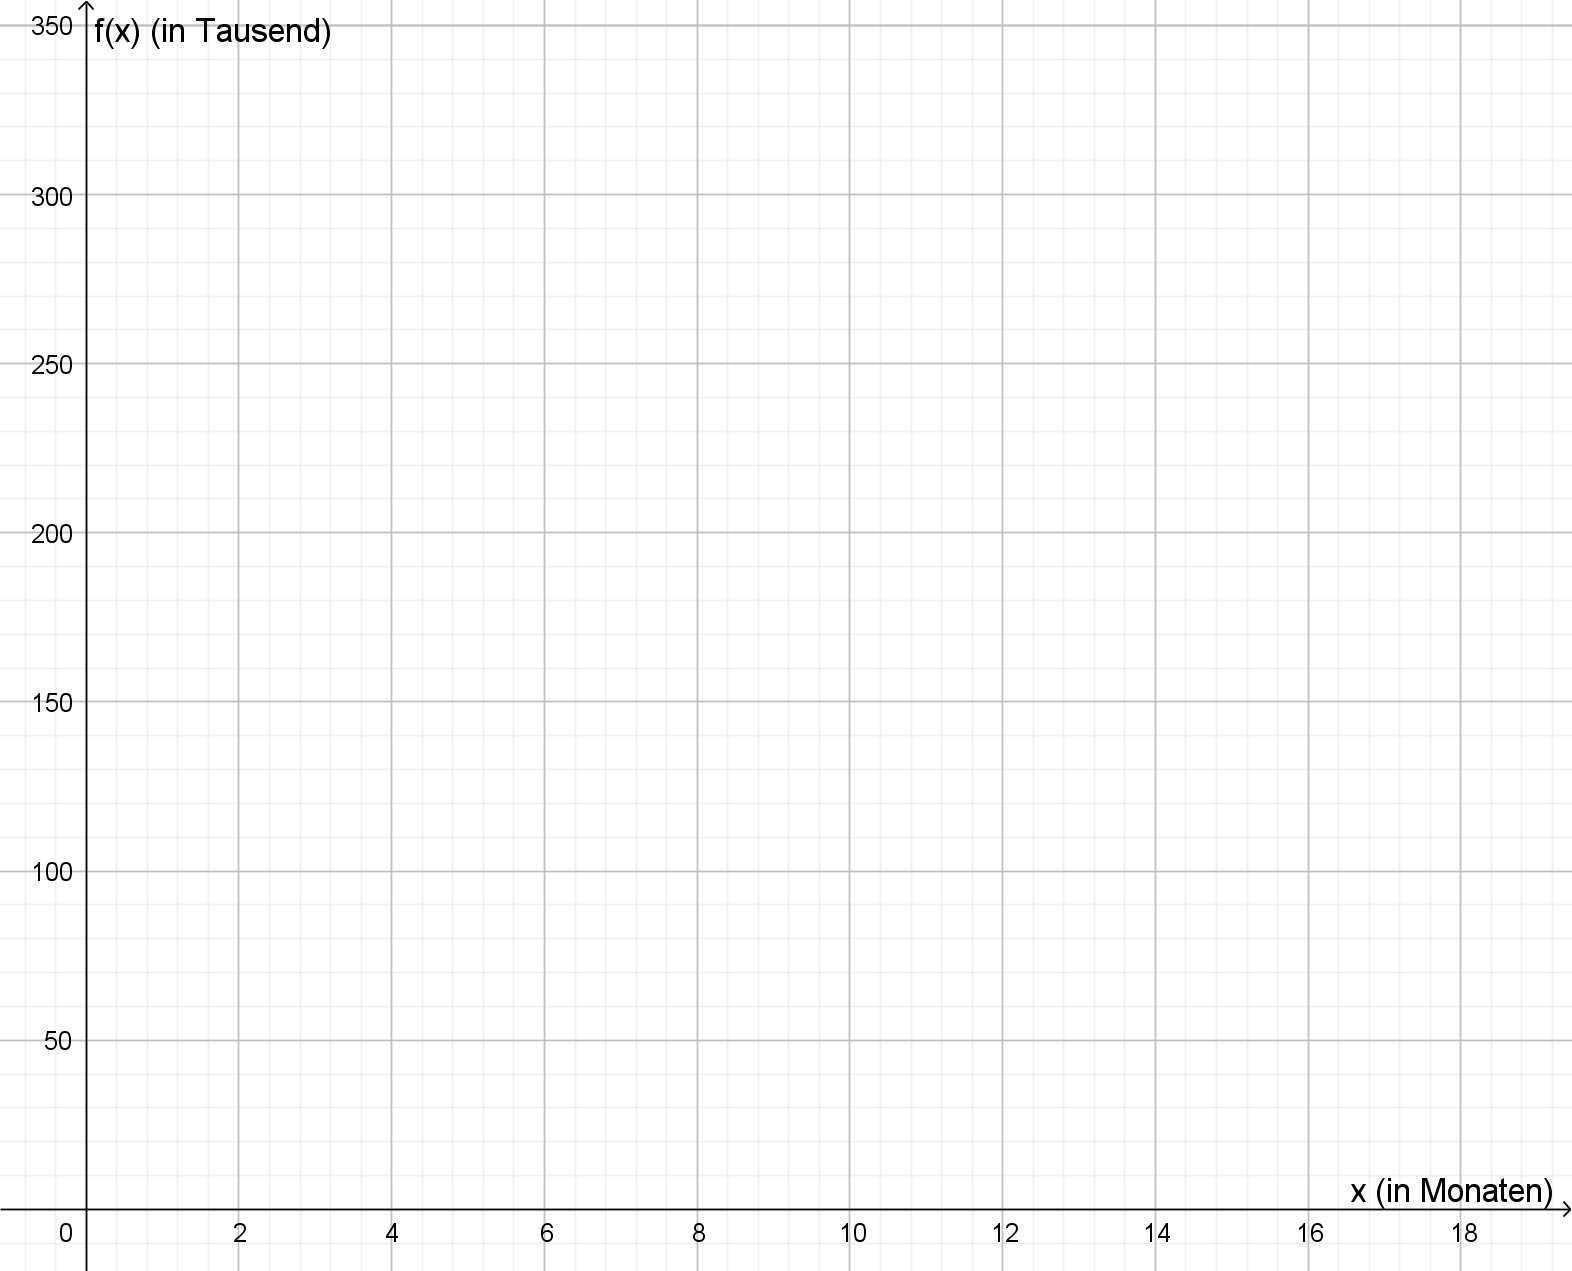
\includegraphics[width=\textwidth]{../99_Bilder/KoordLeer.png}
		\end{framed}
		\newpage
		\begin{framed}
			\noindent
			Mit steigender Zahl der Krypto-Miner wurden auch die Anwender aufmerksamer und starteten Gegenmaßnahmen. Die Entwicklung der Anzahl der von Krypto-Miner-Opfer (befallene Computer) kann durch \(\mathbf{f(x) = (392-0,29x^2)\cdot{}e^{0.25x}}\) verdeutlicht werden.\\
			(\(x\) Monate nach Ausbruch/Feststellung; \(x = 0\) entspricht September 2016; \(f(x)\) Anzahl befallener Computer in Tausend)\\
			\rule{\textwidth}{0.1pt}
			\noindent
			Das Bundesamt für Sicherheit in der Informationstechnik (BSI) möchte im Rahmen der Aufklärung über Krypto-Mining einen informativen Flyer mit den Eckdaten der Entwicklung veröffentlichen.\\
			% f(0)
			(a) Bestimmen Sie zunächst die Anzahl der zu Beginn befallenen Computer.\\
			% f'(x) = 0
			(b) Berechnen Sie den Zeitpunkt des höchsten Befalls und interpretieren diesen Situationsbedingt.\\
			% f''(x) = 0
			(c) Bestimmen Sie den Zeitpunkt, zu welchem die Anzahl der Neubefälle ihr Minimum bzw. ihr Maximum erreicht.\\
			Treffen Sie eine fundierte Aussage über die Entwicklung der Neubefälle \textbf{vor} und \textbf{nach} diesem Zeitpunkt.\\
			% f(x) = 0
			(d) Wie viele Monate nach Beginn der Gegenmaßnahmen kann mit Sicherheit gesagt werden, dass kein Computer befallen ist?
		\end{framed}
		\begin{framed}
			\noindent
			Verdeutlichen Sie die Entwicklung in einem Graphen!\\
			\par\noindent
			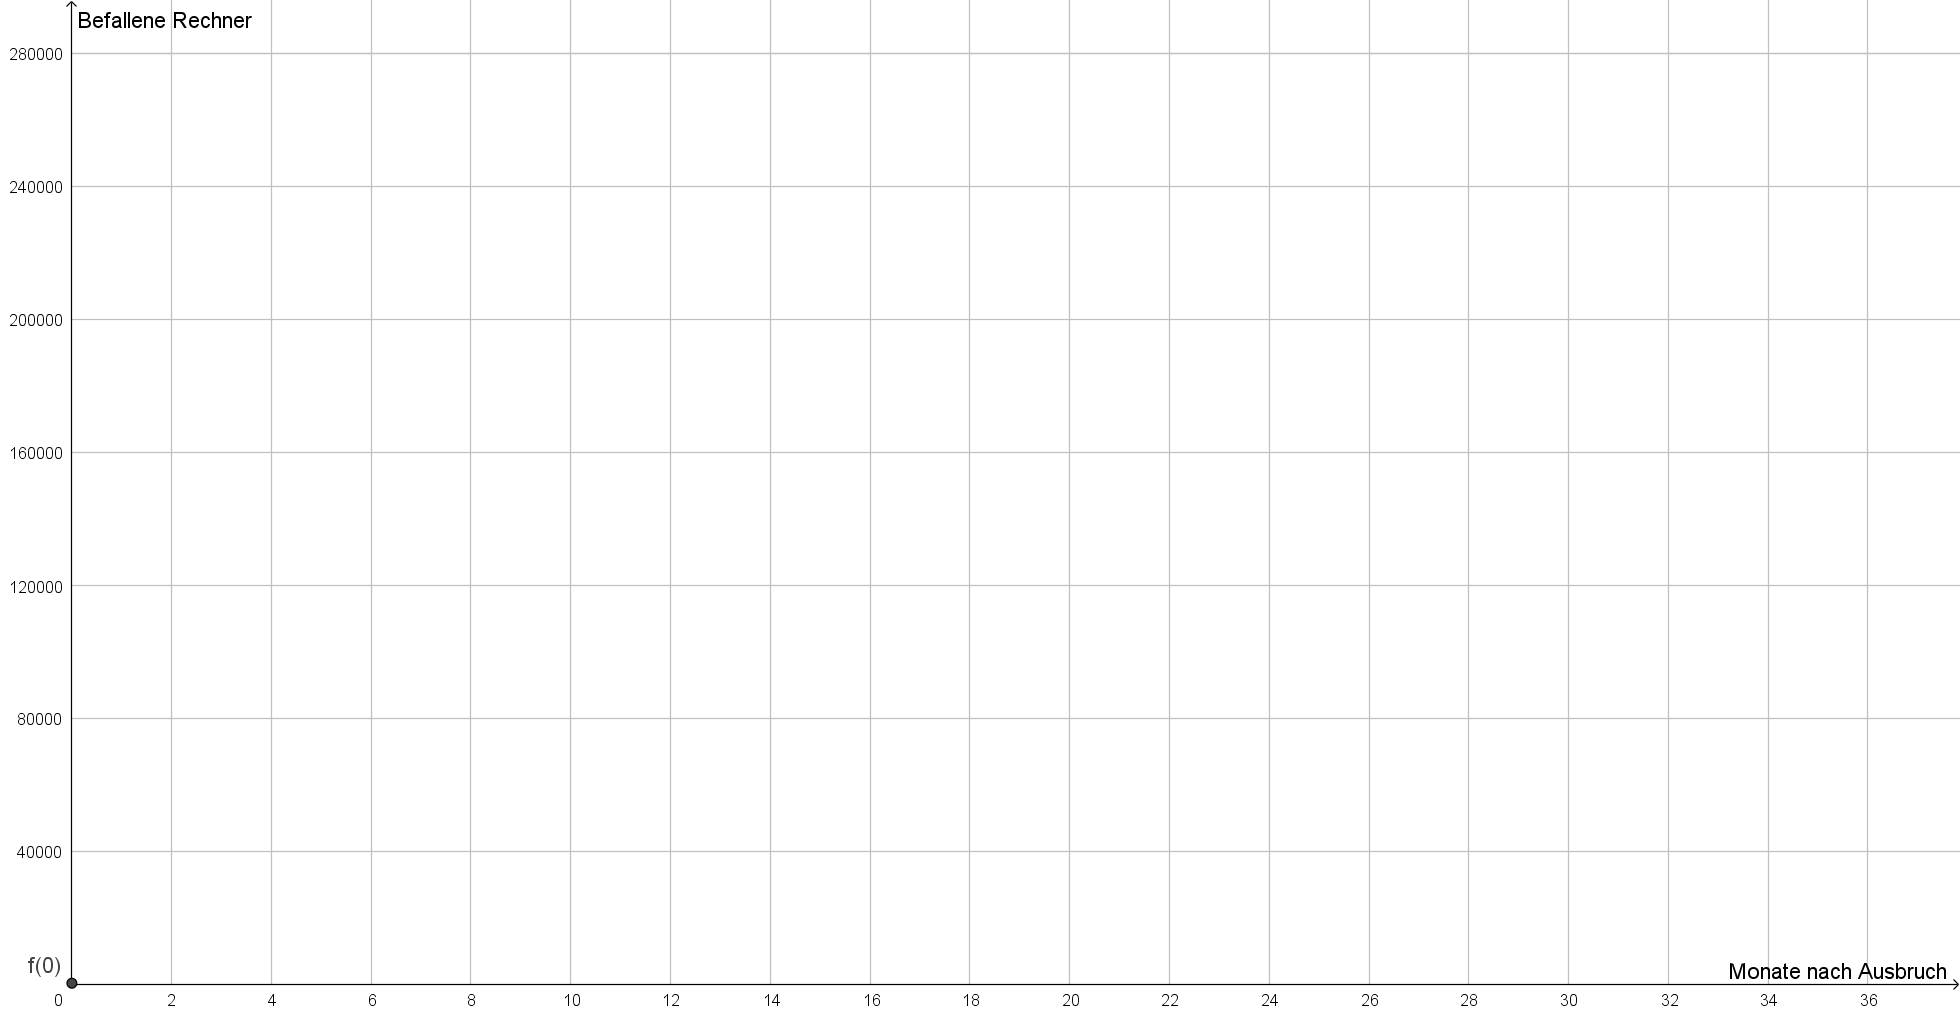
\includegraphics[width=0.86\textwidth]{../99_Bilder/KoordLeer_2.png}
		\end{framed}
	\end{worksheet}
\end{document}